\documentclass[11pt,a4paper]{article}

% ── Packages ──────────────────────────────────────────────────────────────────
\usepackage[utf8]{inputenc}
\usepackage[T1]{fontenc}
\usepackage{lmodern}
\usepackage[margin=2.5cm]{geometry}
\usepackage{graphicx}
\usepackage{xcolor}
\usepackage{hyperref}
\usepackage{listings}
\usepackage{booktabs}
\usepackage{longtable}
\usepackage{amsmath,amssymb}
\usepackage{tikz}
\usetikzlibrary{arrows.meta,positioning,shapes.geometric,calc,fit}
\usepackage{fancyhdr}
\usepackage{enumitem}
\usepackage{caption}
\usepackage{float}
\usepackage{tcolorbox}
\tcbuselibrary{listings,skins,breakable}
\usepackage{multicol}
\usepackage{parskip}

% ── Colors ────────────────────────────────────────────────────────────────────
\definecolor{codebackground}{RGB}{245,245,248}
\definecolor{codeborder}{RGB}{200,200,210}
\definecolor{keywordcolor}{RGB}{0,100,170}
\definecolor{stringcolor}{RGB}{160,32,32}
\definecolor{commentcolor}{RGB}{100,130,100}
\definecolor{highconf}{RGB}{0,120,60}
\definecolor{lowconf}{RGB}{180,120,0}
\definecolor{missing}{RGB}{180,40,40}
\definecolor{accentblue}{RGB}{30,80,160}
\definecolor{lightblue}{RGB}{230,240,255}
\definecolor{lightyellow}{RGB}{255,252,230}
\definecolor{lightgreen}{RGB}{230,248,235}
\definecolor{lightred}{RGB}{255,235,235}
\definecolor{yamlkey}{RGB}{0,100,170}
\definecolor{yamlval}{RGB}{160,32,32}

% ── Listings ──────────────────────────────────────────────────────────────────
\lstdefinestyle{pythonstyle}{
    language=Python,
    backgroundcolor=\color{codebackground},
    basicstyle=\ttfamily\small,
    keywordstyle=\color{keywordcolor}\bfseries,
    stringstyle=\color{stringcolor},
    commentstyle=\color{commentcolor}\itshape,
    numbers=left,
    numberstyle=\tiny\color{gray},
    numbersep=8pt,
    frame=single,
    rulecolor=\color{codeborder},
    breaklines=true,
    breakatwhitespace=false,
    showstringspaces=false,
    tabsize=4,
    captionpos=b,
    xleftmargin=2em,
    framexleftmargin=1.5em,
    aboveskip=1em,
    belowskip=1em,
}

\lstdefinestyle{bashstyle}{
    language=bash,
    backgroundcolor=\color{codebackground},
    basicstyle=\ttfamily\small,
    keywordstyle=\color{keywordcolor}\bfseries,
    stringstyle=\color{stringcolor},
    commentstyle=\color{commentcolor}\itshape,
    frame=single,
    rulecolor=\color{codeborder},
    breaklines=true,
    showstringspaces=false,
    tabsize=4,
    captionpos=b,
    xleftmargin=1em,
    framexleftmargin=0.5em,
    aboveskip=1em,
    belowskip=1em,
}

\lstdefinestyle{yamlstyle}{
    backgroundcolor=\color{codebackground},
    basicstyle=\ttfamily\small,
    frame=single,
    rulecolor=\color{codeborder},
    breaklines=true,
    showstringspaces=false,
    tabsize=2,
    captionpos=b,
    xleftmargin=1em,
    framexleftmargin=0.5em,
    aboveskip=1em,
    belowskip=1em,
    commentstyle=\color{commentcolor}\itshape,
    morecomment=[l]{\#},
}

\lstset{style=pythonstyle}

% ── Tcolorbox styles ─────────────────────────────────────────────────────────
\newtcolorbox{conceptbox}[1][]{
    colback=lightblue,colframe=accentblue,fonttitle=\bfseries,
    title={#1},breakable,arc=2mm,boxrule=0.5mm,
}
\newtcolorbox{warningbox}[1][]{
    colback=lightyellow,colframe=orange!80!black,fonttitle=\bfseries,
    title={#1},breakable,arc=2mm,boxrule=0.5mm,
}
\newtcolorbox{notebox}[1][]{
    colback=lightgreen,colframe=highconf,fonttitle=\bfseries,
    title={#1},breakable,arc=2mm,boxrule=0.5mm,
}

% ── Headers/Footers ──────────────────────────────────────────────────────────
\pagestyle{fancy}
\fancyhf{}
\fancyhead[L]{\small\textit{Ancestral Allele Polarization --- \texttt{ancify} Package}}
\fancyhead[R]{\small\textit{v1.0}}
\fancyfoot[C]{\thepage}
\renewcommand{\headrulewidth}{0.4pt}
\renewcommand{\footrulewidth}{0.4pt}

\hypersetup{
    colorlinks=true,linkcolor=accentblue,
    urlcolor=accentblue,citecolor=accentblue,
}

% ══════════════════════════════════════════════════════════════════════════════
\begin{document}

% ── Title Page ────────────────────────────────────────────────────────────────
\begin{titlepage}
\centering
\vspace*{2.5cm}
{\Huge\bfseries\texttt{ancify}\par}
\vspace{0.5cm}
{\LARGE Ancestral Allele Polarization\\[0.2em]Pipeline for Any Species\par}
\vspace{1.5cm}
{\large A species-agnostic, config-driven Python package\\for inferring ancestral alleles using outgroup alignments\par}
\vspace{2cm}
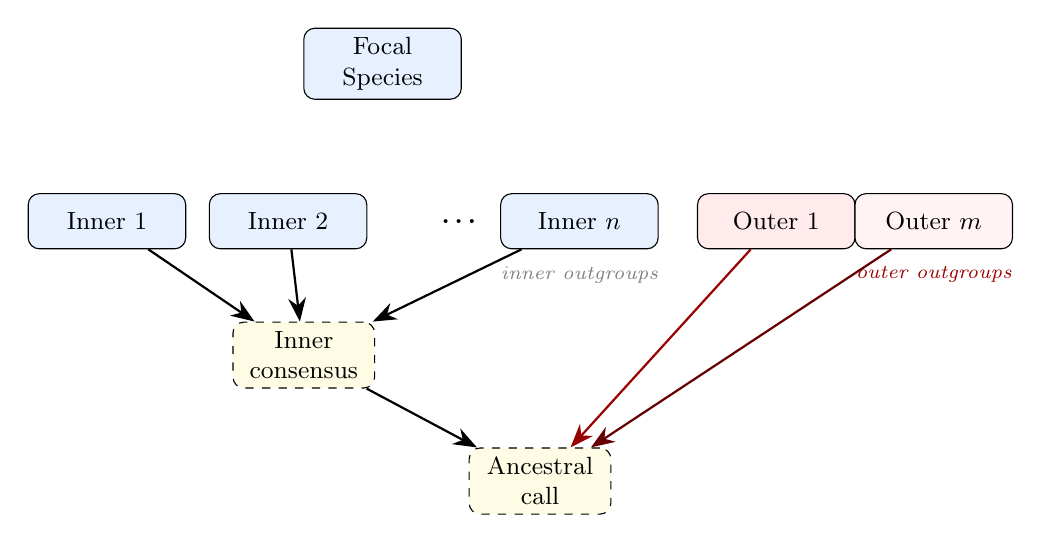
\begin{tikzpicture}[
    every node/.style={font=\small},
    species/.style={draw, rounded corners, fill=lightblue, minimum width=2cm, minimum height=0.7cm, align=center},
    ancestor/.style={draw, rounded corners, fill=lightyellow, minimum width=1.8cm, minimum height=0.6cm, align=center, dashed},
    arr/.style={-{Stealth[length=3mm]}, thick}
]
    \node[species] (focal) at (0,0.5) {Focal\\Species};
    \node[species] (i1) at (-3.5,-1.5) {Inner 1};
    \node[species] (i2) at (-1.2,-1.5) {Inner 2};
    \node (dots) at (1,-1.5) {\bfseries\ldots};
    \node[species] (iN) at (2.5,-1.5) {Inner $n$};
    \node[species, fill=lightred] (o1) at (5,-1.5) {Outer 1};
    \node[species, fill=lightred!60] (oM) at (7,-1.5) {Outer $m$};

    \node[ancestor] (inner) at (-1,-3.2) {Inner\\consensus};
    \node[ancestor] (anc) at (2,-4.8) {Ancestral\\call};

    \draw[arr] (i1) -- (inner);
    \draw[arr] (i2) -- (inner);
    \draw[arr] (iN) -- (inner);
    \draw[arr, red!60!black] (o1) -- (anc);
    \draw[arr, red!40!black] (oM) -- (anc);
    \draw[arr] (inner) -- (anc);

    \node[below=0.1cm of iN, font=\scriptsize\itshape, text=gray] {inner outgroups};
    \node[below=0.1cm of oM, font=\scriptsize\itshape, text=red!60!black] {outer outgroups};
\end{tikzpicture}
\vfill
{\small Version 1.0 \quad---\quad Generated: \today\par}
\end{titlepage}

% ── TOC ───────────────────────────────────────────────────────────────────────
\tableofcontents
\newpage


% ══════════════════════════════════════════════════════════════════════════════
\section{Introduction}
\label{sec:intro}

\subsection{Why Polarize Variants?}

In population genetics, most analyses of the \textbf{site frequency spectrum} (SFS) require knowing whether an allele is \emph{ancestral} (inherited from the common ancestor) or \emph{derived} (arose by mutation).  Without polarization, the SFS is \emph{folded}---one cannot distinguish a rare derived allele from a rare ancestral allele---which limits the power of tests for selection, demographic inference, and mutation-rate estimation.

Polarization is required for:
\begin{itemize}[leftmargin=2em]
    \item \textbf{Unfolded SFS}: used by $\partial$a$\partial$i, moments, \texttt{mushi}, and similar demographic inference tools.
    \item \textbf{Tests of selection}: McDonald--Kreitman, Fay \& Wu's $H$, $D_n/D_s$, etc.
    \item \textbf{Ancestral recombination graphs}: correct orientation of mutations on genealogies.
    \item \textbf{Mutation spectra}: directional mutation-rate estimation requires knowing which allele is ancestral.
\end{itemize}

\subsection{The Outgroup Approach}

The standard approach compares the focal species to one or more \textbf{outgroup} species.  If an outgroup carries allele $X$ and the focal species is polymorphic for $X$ and $Y$, parsimony suggests $X$ is ancestral.  Using \emph{multiple} outgroups reduces misinference from back-mutations, convergent evolution, and incomplete lineage sorting (ILS).

\subsection{What This Package Does}

The \texttt{ancify} package generalises this logic into a species-agnostic, config-driven pipeline:

\begin{enumerate}[leftmargin=2em]
    \item \textbf{Phase 1 --- Projection}: converts pairwise net-AXT alignments from any number of outgroup species into FASTA files in focal-species coordinates.
    \item \textbf{Phase 2 --- Ancestral calling}: infers the ancestral allele at every position using a two-tier inner/outer outgroup voting scheme with case-encoded confidence.
    \item \textbf{Phase 3 --- Evaluation} (optional): compares the calls against a reference ancestral sequence and/or VCF variant data.
\end{enumerate}

The pipeline works for \textbf{any focal species} for which pairwise net-AXT alignments to outgroup species are available (typically from the UCSC Genome Browser).


% ══════════════════════════════════════════════════════════════════════════════
\section{Biological Background}
\label{sec:background}

\subsection{Inner vs.\ Outer Outgroups}

The pipeline partitions outgroup species into two tiers:

\begin{description}[leftmargin=2em, labelwidth=3.5cm]
    \item[Inner outgroup] One or more \emph{closely related} species.  A majority vote among them produces the \textbf{inner consensus}.  Because these species diverged recently from the focal species, most of their genome is identical to the true ancestral state.
    \item[Outer outgroup] One or more \emph{distantly related} species.  They serve as an independent check: if the inner consensus agrees with the outer outgroup, the call is made with high confidence.
\end{description}

\begin{conceptbox}[Example: Human Polarization]
For \textit{Homo sapiens} (hg38):
\begin{itemize}
    \item Inner: bonobo ($\sim$6\,Mya), chimpanzee ($\sim$6\,Mya), gorilla ($\sim$9\,Mya)
    \item Outer: rhesus macaque ($\sim$25\,Mya)
\end{itemize}
If all three great apes agree on allele \texttt{A} and macaque also carries \texttt{A}, the ancestral call is \texttt{A} with high confidence.
\end{conceptbox}

\begin{conceptbox}[Example: Drosophila Polarization]
For \textit{D.~melanogaster} (dm6):
\begin{itemize}
    \item Inner: \textit{D.~simulans}, \textit{D.~sechellia}
    \item Outer: \textit{D.~yakuba}
\end{itemize}
Same algorithm, different species tree.
\end{conceptbox}

\subsection{Net Alignments and the AXT Format}

The pipeline uses \textbf{net alignments} from the UCSC Genome Browser---one-to-one best-chain pairwise alignments stored in \textbf{AXT format}.  Each alignment block consists of four lines:

\begin{enumerate}
    \item Header: index, target chromosome, start, end, query chromosome, start, end, strand, score.
    \item Target (focal) aligned sequence (with gap characters \texttt{-}).
    \item Query (outgroup) aligned sequence.
    \item Blank separator.
\end{enumerate}

These files can be downloaded from UCSC for hundreds of species pairs.


% ══════════════════════════════════════════════════════════════════════════════
\section{Installation}
\label{sec:install}

\subsection{From Source}

\begin{lstlisting}[style=bashstyle]
cd ancify/
pip install .
\end{lstlisting}

This installs the \texttt{ancify} command-line tool and the \texttt{ancify} Python package.

\subsection{With Evaluation Dependencies}

The evaluation phase (Phase~3) requires \texttt{scikit-allel} and \texttt{matplotlib}:

\begin{lstlisting}[style=bashstyle]
pip install '.[evaluate]'
\end{lstlisting}

\subsection{Core Dependencies}

\begin{table}[H]
\centering
\caption{Package dependencies.}
\begin{tabular}{lll}
\toprule
\textbf{Package} & \textbf{Purpose} & \textbf{Required?} \\
\midrule
\texttt{pyyaml} & Configuration file parsing & Yes \\
\texttt{numpy} & Array operations in evaluation & Yes \\
\texttt{scikit-allel} & VCF reading (Phase~3) & Optional \\
\texttt{matplotlib} & Plotting (Phase~3) & Optional \\
\bottomrule
\end{tabular}
\end{table}


% ══════════════════════════════════════════════════════════════════════════════
\section{Package Architecture}
\label{sec:architecture}

\subsection{Module Layout}

\begin{lstlisting}[style=bashstyle, caption={Package file structure.}]
ancify/                       # project root
|-- pyproject.toml            # build metadata & dependencies
|-- example_configs/
|   |-- hg38_bcgm.yaml       # human worked example
|   |-- mouse_example.yaml   # mouse hypothetical example
|   |-- drosophila_example.yaml
|   |-- brassica_rapa_example.yaml
|-- ancify/                   # importable Python package
    |-- __init__.py
    |-- __main__.py           # python -m ancify
    |-- cli.py                # command-line interface
    |-- config.py             # YAML config loading & validation
    |-- utils.py              # FASTA I/O, majority_vote, helpers
    |-- project.py            # Phase 1: coordinate projection
    |-- ancestral.py          # Phase 2: ancestral state inference
    |-- evaluate.py           # Phase 3: evaluation & QC
\end{lstlisting}

\subsection{Three-Phase Pipeline}

\begin{figure}[H]
\centering
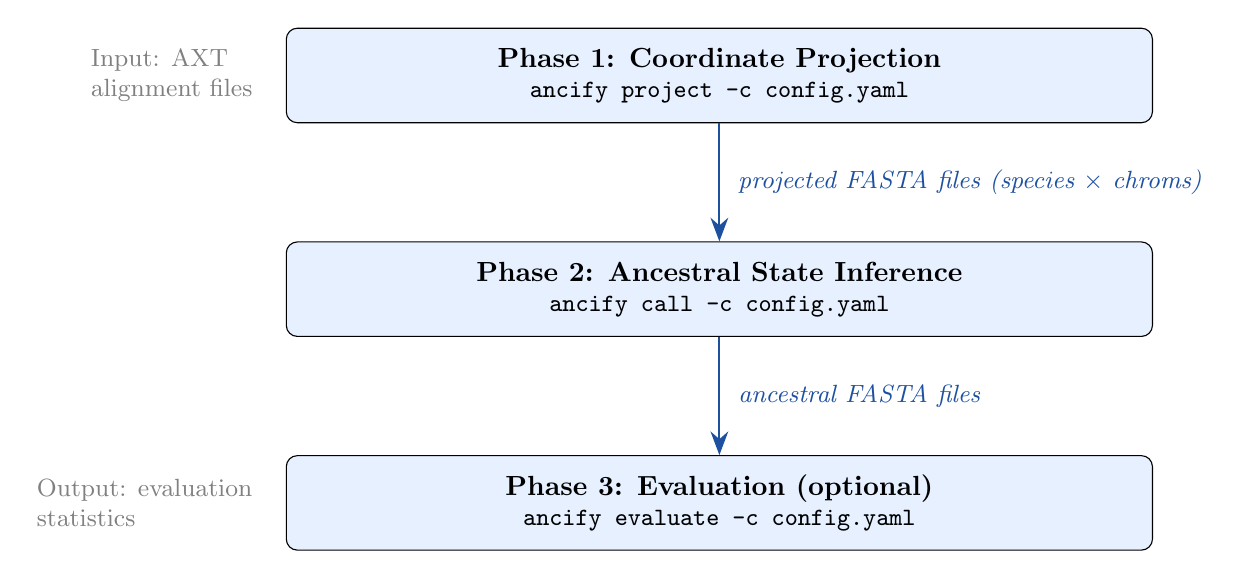
\begin{tikzpicture}[
    node distance=1.2cm and 2cm,
    phase/.style={draw, rounded corners, fill=lightblue, minimum width=11cm,
                  minimum height=1.2cm, align=center, font=\bfseries},
    detail/.style={font=\small, align=left},
    arr/.style={-{Stealth[length=3mm]}, thick, accentblue},
]
    \node[phase] (p1) {Phase 1: Coordinate Projection\\[-0.1em]
        \normalfont\small\texttt{ancify project -c config.yaml}};
    \node[phase, below=1.5cm of p1] (p2) {Phase 2: Ancestral State Inference\\[-0.1em]
        \normalfont\small\texttt{ancify call -c config.yaml}};
    \node[phase, below=1.5cm of p2] (p3) {Phase 3: Evaluation (optional)\\[-0.1em]
        \normalfont\small\texttt{ancify evaluate -c config.yaml}};

    \draw[arr] (p1) -- (p2) node[midway, right, detail]
        {~\textit{projected FASTA files (species $\times$ chroms)}};
    \draw[arr] (p2) -- (p3) node[midway, right, detail]
        {~\textit{ancestral FASTA files}};

    \node[left=0.3cm of p1, detail, text=gray] {Input: AXT\\alignment files};
    \node[left=0.3cm of p3, detail, text=gray] {Output: evaluation\\statistics};
\end{tikzpicture}
\caption{Three-phase pipeline, each invocable independently or together via \texttt{ancify run}.}
\label{fig:arch}
\end{figure}


% ══════════════════════════════════════════════════════════════════════════════
\section{Configuration}
\label{sec:config}

All pipeline behaviour is controlled by a single \textbf{YAML configuration file}.  Generate a template with:

\begin{lstlisting}[style=bashstyle]
ancify init -o config.yaml
\end{lstlisting}

\subsection{Configuration Reference}

\begin{lstlisting}[style=yamlstyle, caption={Annotated configuration file.}]
# Informal label for the focal species.
focal_species: human

# Tab-separated file: chrom_name <TAB> length [<TAB> ...]
chromosome_lengths: chromoLens.txt

# Optional: restrict to specific chromosomes.
# If omitted, all entries in the lengths file are used.
chromosomes:
  - chr1
  - chr2
  - chrX

outgroups:
  # Inner: closely related species (majority vote).
  inner:
    - name: bonobo
      alignment: hg38.panPan3.net.axt.gz
    - name: chimp
      alignment: hg38.panTro6.net.axt.gz
    - name: gorilla
      alignment: hg38.gorGor6.net.axt.gz
  # Outer: distantly related species (independent check).
  outer:
    - name: macaque
      alignment: hg38.rheMac10.net.axt.gz

# Intermediate files go here (projected/ subdirectory).
work_dir: .

# Final ancestral FASTA files go here.
output_dir: ./ancestral_calls

# Minimum allele count for the majority-vote consensus.
min_inner_freq: 1
min_outer_freq: 1

# Parallel workers (one chromosome per worker).
num_cpus: 24

# Optional evaluation block.
evaluation:
  reference_dir: ./reference_ancestral/
  # {chrom} = full name, {chrom_id} = without "chr" prefix
  reference_pattern: "ancestor_{chrom_id}.fa"
  vcf_dir: ./vcf/
  vcf_pattern: "variants.{chrom}.vcf.gz"
\end{lstlisting}

\subsection{Key Configuration Fields}

\begin{table}[H]
\centering
\caption{Configuration fields and their meaning.}
\label{tab:config}
\begin{tabular}{p{3.5cm}p{2cm}p{7.5cm}}
\toprule
\textbf{Field} & \textbf{Required} & \textbf{Description} \\
\midrule
\texttt{focal\_species} & Yes & Label for the focal species (cosmetic). \\
\texttt{chromosome\_lengths} & Yes & Path to tab-separated lengths file. \\
\texttt{chromosomes} & No & Subset of chromosomes to process; defaults to all. \\
\texttt{outgroups.inner} & Yes & List of inner outgroup species (name + alignment path). \\
\texttt{outgroups.outer} & Yes & List of outer outgroup species (name + alignment path). \\
\texttt{work\_dir} & No & Working directory for projected sequences (default: \texttt{.}). \\
\texttt{output\_dir} & No & Output directory for ancestral FASTAs (default: \texttt{./ancestral\_calls}). \\
\texttt{min\_inner\_freq} & No & Minimum count for inner majority vote (default: 1). \\
\texttt{min\_outer\_freq} & No & Minimum count for outer majority vote (default: 1). \\
\texttt{num\_cpus} & No & Parallel workers (default: 4). \\
\texttt{evaluation} & No & Optional block for Phase~3 settings. \\
\bottomrule
\end{tabular}
\end{table}

\subsection{Pattern Placeholders}

Evaluation filename patterns support two placeholders:
\begin{itemize}[leftmargin=2em]
    \item \texttt{\{chrom\}} --- the full chromosome name as it appears in the config (e.g.\ \texttt{chr1}, \texttt{2L}).
    \item \texttt{\{chrom\_id\}} --- the name with any leading \texttt{chr} prefix stripped (e.g.\ \texttt{1}, \texttt{X}).
\end{itemize}


% ══════════════════════════════════════════════════════════════════════════════
\section{Phase 1: Coordinate Projection}
\label{sec:phase1}

\subsection{Purpose}

Transforms each outgroup's pairwise alignment (AXT format) into a FASTA file where every position corresponds to a position in the focal-species reference.  Unaligned positions are filled with \texttt{N}.

\subsection{Algorithm (\texttt{ancify.project})}

\begin{enumerate}[leftmargin=2em]
    \item Load focal-species chromosome lengths from the config.
    \item For each outgroup $\times$ chromosome combination:
    \begin{enumerate}
        \item Allocate a byte array of length $L$ (chromosome length), pre-filled with \texttt{N}.
        \item Stream through the AXT file.  For each alignment block matching the target chromosome, walk the aligned human sequence position by position:
        \begin{itemize}
            \item If the focal character is a nucleotide (\texttt{A/T/C/G/N}), store the corresponding outgroup character at the focal coordinate.
            \item If the focal character is a gap (\texttt{-}), skip (insertion in the outgroup, not in focal coordinates).
        \end{itemize}
        \item Write the resulting sequence as a FASTA file.
    \end{enumerate}
\end{enumerate}

\begin{lstlisting}[caption={Core projection logic (simplified from \texttt{project.py}).}]
seq = bytearray(b"N" * chrom_length)
with open(axt_path, "rt") as f:
    for block in parse_axt_blocks(f):
        if block.target_chrom == target_chrom:
            pos = block.start
            for h, q in zip(block.target_seq, block.query_seq):
                if h.upper() in "ATCGN":
                    seq[pos - 1] = ord(q)
                    pos += 1
return seq.decode("ascii")
\end{lstlisting}

\subsection{Output}

Phase~1 creates \texttt{<work\_dir>/projected/<species>/<chrom>.fa} for every outgroup species and chromosome.

Parallelization uses Python's \texttt{ProcessPoolExecutor} with one worker per task (species $\times$ chromosome).


% ══════════════════════════════════════════════════════════════════════════════
\section{Phase 2: Ancestral State Inference}
\label{sec:phase2}

\subsection{The Generalized Algorithm}

For each genomic position, the algorithm performs two majority votes and then compares:

\begin{figure}[H]
\centering
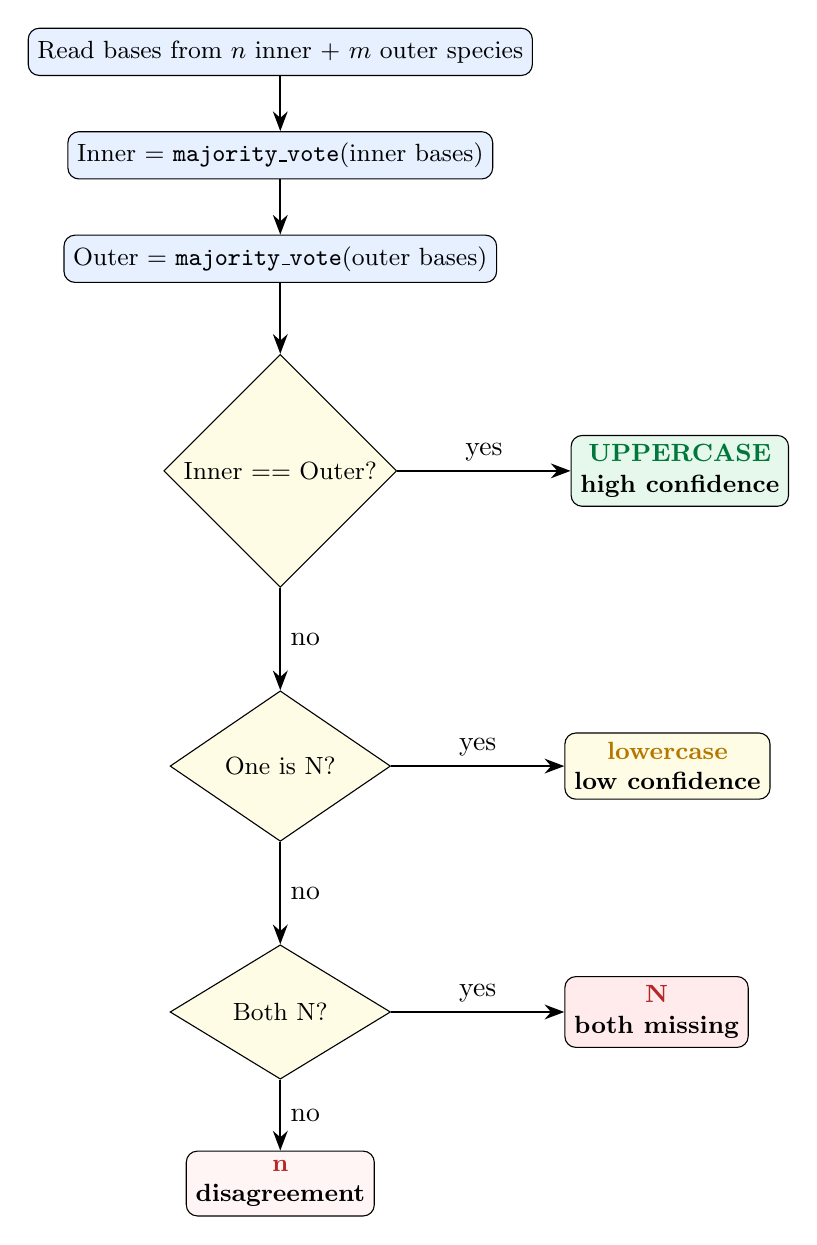
\begin{tikzpicture}[
    node distance=0.9cm,
    decision/.style={diamond, draw, fill=lightyellow, minimum width=2.8cm,
                     minimum height=0.9cm, align=center, font=\small, inner sep=2pt},
    process/.style={rectangle, draw, rounded corners, fill=lightblue,
                    minimum width=2.5cm, minimum height=0.6cm, align=center, font=\small},
    result/.style={rectangle, draw, rounded corners, minimum width=2cm,
                   minimum height=0.6cm, align=center, font=\small\bfseries},
    arr/.style={-{Stealth[length=2.5mm]}, thick},
]
    \node[process] (start) {Read bases from $n$ inner +{} $m$ outer species};
    \node[process, below=0.7cm of start] (inner) {Inner = \texttt{majority\_vote}(inner bases)};
    \node[process, below=0.7cm of inner] (outer) {Outer = \texttt{majority\_vote}(outer bases)};
    \node[decision, below=0.9cm of outer] (agree) {Inner == Outer?};

    \node[result, fill=lightgreen, right=2.2cm of agree] (high)
        {\textcolor{highconf}{UPPERCASE}\\high confidence};

    \node[decision, below=1.3cm of agree] (onemiss) {One is N?};

    \node[result, fill=lightyellow, right=2.2cm of onemiss] (low)
        {\textcolor{lowconf}{lowercase}\\low confidence};

    \node[decision, below=1.3cm of onemiss] (bothmiss) {Both N?};

    \node[result, fill=lightred, right=2.2cm of bothmiss] (N)
        {\textcolor{missing}{N}\\both missing};

    \node[result, fill=lightred!50, below=0.9cm of bothmiss] (n)
        {\textcolor{missing}{n}\\disagreement};

    \draw[arr] (start) -- (inner);
    \draw[arr] (inner) -- (outer);
    \draw[arr] (outer) -- (agree);
    \draw[arr] (agree) -- node[above] {yes} (high);
    \draw[arr] (agree) -- node[right] {no} (onemiss);
    \draw[arr] (onemiss) -- node[above] {yes} (low);
    \draw[arr] (onemiss) -- node[right] {no} (bothmiss);
    \draw[arr] (bothmiss) -- node[above] {yes} (N);
    \draw[arr] (bothmiss) -- node[right] {no} (n);
\end{tikzpicture}
\caption{Decision flowchart for the generalized ancestral calling algorithm.}
\label{fig:algorithm}
\end{figure}

\subsection{Core Function}

\begin{lstlisting}[caption={\texttt{call\_ancestral\_base()} from \texttt{ancestral.py}.}]
def call_ancestral_base(inner_bases, outer_bases,
                        min_inner_freq=1, min_outer_freq=1):
    inner = majority_vote(inner_bases, min_inner_freq)
    outer = majority_vote(outer_bases, min_outer_freq)

    if inner != "N" and inner == outer:
        return inner              # HIGH confidence (uppercase)
    if inner == "N" and outer != "N":
        return outer.lower()      # LOW confidence (lowercase)
    if inner != "N" and outer == "N":
        return inner.lower()      # LOW confidence (lowercase)
    if inner == "N" and outer == "N":
        return "N"                # Both missing
    return "n"                    # Disagreement
\end{lstlisting}

\subsection{The \texttt{majority\_vote()} Function}

\begin{lstlisting}[caption={\texttt{majority\_vote()} from \texttt{utils.py}.}]
VALID_ALLELES = ("A", "C", "G", "T")

def majority_vote(bases, min_freq=1):
    upper = [b.upper() for b in bases]
    counts = {a: upper.count(a) for a in VALID_ALLELES}
    best = max(VALID_ALLELES, key=lambda a: counts[a])
    if counts[best] < min_freq:
        return "N"
    return best
\end{lstlisting}

Ties are broken in alphabetical order (A, C, G, T) for reproducibility.  The function works for any number of input species ($n \geq 1$).

\subsection{Output Encoding}

\begin{table}[H]
\centering
\caption{Confidence encoding in the output FASTA.}
\label{tab:encoding}
\begin{tabular}{cll}
\toprule
\textbf{Character} & \textbf{Confidence} & \textbf{Condition} \\
\midrule
\texttt{A}, \texttt{C}, \texttt{G}, \texttt{T} & High & Inner and outer outgroups agree \\
\texttt{a}, \texttt{c}, \texttt{g}, \texttt{t} & Low & Only one outgroup tier has data \\
\texttt{n} (lowercase) & Unresolved & Inner and outer disagree \\
\texttt{N} (uppercase) & Missing & Both tiers lack data \\
\bottomrule
\end{tabular}
\end{table}

\begin{conceptbox}[Why Letter Case?]
Using uppercase for high-confidence and lowercase for low-confidence calls is a compact encoding within standard FASTA format.  Downstream tools can filter by confidence level: for stringent analyses, restrict to uppercase bases (inner--outer agreement); for maximum coverage, include lowercase as well.  This convention is compatible with the Ensembl EPO ancestral sequences.
\end{conceptbox}


% ══════════════════════════════════════════════════════════════════════════════
\section{Phase 3: Evaluation}
\label{sec:phase3}

\subsection{Available Metrics}

The evaluation module computes three categories of metrics (the latter two are optional):

\begin{description}[leftmargin=2em]
    \item[Coverage statistics] (always): proportion of high-confidence, low-confidence, and missing positions.
    \item[Reference comparison] (optional): agreement rate between the pipeline's calls and a reference ancestral sequence (e.g.\ Ensembl EPO).
    \item[VCF comparison] (optional): concordance of ancestral calls with REF/ALT alleles at known variant sites.
\end{description}

\subsection{Output}

For each chromosome, a summary file is written to \texttt{<output\_dir>/evaluation/<chrom>.evaluation.txt} with sections:

\begin{lstlisting}[style=bashstyle, caption={Example evaluation output.}]
[coverage]
  total_positions: 248956422
  high_confidence: 197145832
  low_confidence: 25203651
  missing: 26606939
  prop_nonmissing: 0.8931
  prop_high_confidence: 0.7918

[reference_comparison]
  test_nonmissing: 0.7912
  ref_nonmissing: 0.9016
  both_nonmissing: 5234112
  agreement_rate: 0.9992
  disagreement_rate: 0.0008

[vcf_comparison]
  num_variants: 6102435
  prop_nonmissing: 0.8965
  matches_ref: 0.9453
  matches_alt: 0.0494
  matches_either: 0.9948
\end{lstlisting}


% ══════════════════════════════════════════════════════════════════════════════
\section{Command-Line Interface}
\label{sec:cli}

\subsection{Available Commands}

\begin{table}[H]
\centering
\caption{CLI commands.}
\begin{tabular}{lp{9cm}}
\toprule
\textbf{Command} & \textbf{Description} \\
\midrule
\texttt{ancify init [-o FILE]} & Generate a template configuration file. \\
\texttt{ancify project -c CONFIG} & Run Phase~1 (coordinate projection). \\
\texttt{ancify call -c CONFIG} & Run Phase~2 (ancestral calling). \\
\texttt{ancify evaluate -c CONFIG} & Run Phase~3 (evaluation). \\
\texttt{ancify run -c CONFIG} & Run all phases end-to-end. \\
\bottomrule
\end{tabular}
\end{table}

\subsection{Global Options}

\begin{lstlisting}[style=bashstyle]
ancify -v run -c config.yaml      # verbose (debug) logging
ancify run -c config.yaml -n 8    # override num_cpus to 8
\end{lstlisting}

The package can also be invoked as a module:
\begin{lstlisting}[style=bashstyle]
python -m ancify run -c config.yaml
\end{lstlisting}


% ══════════════════════════════════════════════════════════════════════════════
\section{Worked Example: Human (hg38) BCGM}
\label{sec:example_human}

This section walks through the original use case that motivated the package: polarizing the human genome using bonobo, chimpanzee, gorilla, and macaque.

\subsection{Phylogenetic Context}

\begin{figure}[H]
\centering
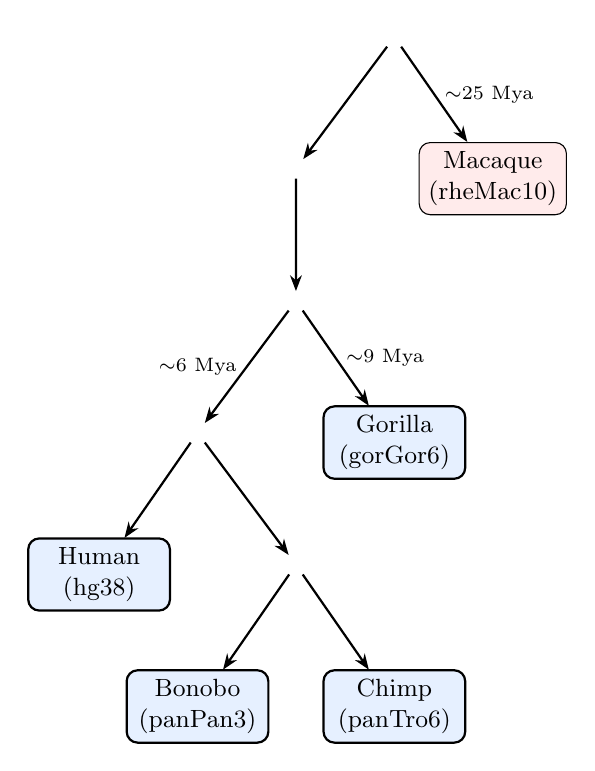
\begin{tikzpicture}[
    level distance=1.8cm, sibling distance=2.5cm,
    edge from parent/.style={draw, thick, -{Stealth[length=2mm]}},
    every node/.style={font=\small},
    species/.style={draw, rounded corners, fill=lightblue,
                    minimum width=1.8cm, minimum height=0.55cm, align=center},
]
    \node[anchor=south] (root) at (0,0) {}
        child {
            node[anchor=south] {}
            child {
                node[anchor=south] {}
                child {
                    node[anchor=south] {}
                    child { node[species] {Human\\(hg38)} }
                    child {
                        node[anchor=south] {}
                        child { node[species] {Bonobo\\(panPan3)} }
                        child { node[species] {Chimp\\(panTro6)} }
                    }
                    edge from parent node[left, font=\scriptsize] {$\sim$6 Mya}
                }
                child { node[species] {Gorilla\\(gorGor6)} edge from parent
                    node[right, font=\scriptsize] {$\sim$9 Mya} }
            }
            edge from parent
        }
        child {
            node[species, fill=lightred] {Macaque\\(rheMac10)}
            edge from parent node[right, font=\scriptsize] {$\sim$25 Mya}
        }
    ;
\end{tikzpicture}
\caption{Great ape phylogeny for the human BCGM pipeline.}
\label{fig:phylogeny}
\end{figure}

\subsection{Configuration}

The example config is provided in \texttt{example\_configs/hg38\_bcgm.yaml}:

\begin{lstlisting}[style=yamlstyle, caption={Key sections of the hg38 BCGM config.}]
focal_species: human
chromosome_lengths: chromoLens.txt

outgroups:
  inner:
    - name: bonobo
      alignment: hg38.panPan3.net.axt.gz
    - name: chimp
      alignment: hg38.panTro6.net.axt.gz
    - name: gorilla
      alignment: hg38.gorGor6.net.axt.gz
  outer:
    - name: macaque
      alignment: hg38.rheMac10.net.axt.gz

output_dir: ./human_ancestor_bcgm
num_cpus: 24

evaluation:
  reference_dir: ./embi_homo_sapiens_ancestor_GRCh38
  reference_pattern: "homo_sapiens_ancestor_{chrom_id}.fa"
  vcf_dir: /path/to/1000genomes/
  vcf_pattern: "ALL.chr{chrom_id}...vcf.gz"
\end{lstlisting}

\subsection{Input Data}

\begin{table}[H]
\centering
\caption{Input alignment files for the human BCGM pipeline.}
\begin{tabular}{llr}
\toprule
\textbf{File} & \textbf{Species} & \textbf{Size} \\
\midrule
\texttt{hg38.panTro6.net.axt.gz} & Chimpanzee & 1.67\,GB \\
\texttt{hg38.panPan3.net.axt.gz} & Bonobo & 1.66\,GB \\
\texttt{hg38.gorGor6.net.axt.gz} & Gorilla & 1.66\,GB \\
\texttt{hg38.rheMac10.net.axt.gz} & Macaque & 1.40\,GB \\
\bottomrule
\end{tabular}
\end{table}

These are downloaded from the UCSC Genome Browser:
\begin{lstlisting}[style=bashstyle]
wget https://hgdownload.soe.ucsc.edu/goldenPath/hg38/\
     vsPanTro6/hg38.panTro6.net.axt.gz
\end{lstlisting}

\subsection{Running the Pipeline}

\begin{lstlisting}[style=bashstyle]
ancify run -c example_configs/hg38_bcgm.yaml
\end{lstlisting}

Or phase by phase:
\begin{lstlisting}[style=bashstyle]
ancify project  -c hg38_bcgm.yaml    # 2-8 hours
ancify call     -c hg38_bcgm.yaml    # 30-60 minutes
ancify evaluate -c hg38_bcgm.yaml    # 20-40 minutes
\end{lstlisting}

\subsection{Evaluation Results}

The BCGM calls have been evaluated against the Ensembl EPO (13-primate) ancestral reference:

\begin{table}[H]
\centering
\caption{BCGM vs.\ Ensembl EPO for selected human chromosomes (high-confidence only).}
\begin{tabular}{lccc}
\toprule
\textbf{Metric} & \textbf{chr1} & \textbf{chr22} & \textbf{chrX} \\
\midrule
Non-missing (BCGM) & 79.1\% & 74.6\% & 44.4\% \\
Non-missing (EMBI) & 90.2\% & 81.2\% & 44.1\% \\
Disagreement rate & 0.083\% & 0.109\% & 3.51\% \\
BCGM matches REF/ALT & 99.6\% & 99.5\% & 99.3\% \\
EMBI matches REF/ALT & 99.5\% & 99.5\% & 100.0\% \\
\bottomrule
\end{tabular}
\end{table}

\begin{notebox}[Key Observations]
\begin{itemize}
    \item BCGM and EMBI agree at $>$99.9\% of autosomal sites where both call.
    \item EMBI has higher coverage because it uses a 13-species multiple alignment.
    \item Including low-confidence calls raises BCGM coverage from $\sim$79\% to $\sim$90\% on chr1 (with disagreement increasing from 0.08\% to 0.57\%).
    \item Both methods achieve $>$99.3\% concordance with 1000G REF/ALT alleles.
\end{itemize}
\end{notebox}


% ══════════════════════════════════════════════════════════════════════════════
\section{Adapting to Other Species}
\label{sec:other_species}

\subsection{What You Need}

To polarize a new focal species you need:

\begin{enumerate}[leftmargin=2em]
    \item \textbf{A reference genome assembly} for the focal species.
    \item \textbf{A chromosome-lengths file}: a tab-separated file with at least two columns (chromosome name, length in bp).
    \item \textbf{Pairwise net-AXT alignment files} for each outgroup species.  These are widely available from the UCSC Genome Browser's download site for many vertebrate and insect assemblies.
    \item \textbf{Phylogenetic knowledge} to decide which species are ``inner'' (closely related) and which are ``outer'' (distantly related).
\end{enumerate}

\subsection{Choosing Inner vs.\ Outer Outgroups}

\begin{warningbox}[Design Guidelines]
\begin{itemize}
    \item \textbf{Inner outgroups} should diverge from the focal species \emph{more recently} than the outer outgroup.  They provide the primary ancestral signal.
    \item \textbf{Outer outgroups} should be \emph{far enough} that convergent substitutions with the inner outgroup are rare.  A divergence of $>$2$\times$ the inner divergence is a useful rule of thumb.
    \item Using $\geq$2 inner outgroups enables majority voting, which is robust to single-species alignment gaps or lineage-specific substitutions.
    \item Multiple outer outgroups can also be used; they undergo their own majority vote.
\end{itemize}
\end{warningbox}

\subsection{Example: Mouse}

\begin{lstlisting}[style=yamlstyle, caption={Hypothetical mouse configuration.}]
focal_species: mouse
chromosome_lengths: mm39.chromLens.txt

outgroups:
  inner:
    - name: rat
      alignment: mm39.rn7.net.axt.gz
  outer:
    - name: rabbit
      alignment: mm39.oryCun2.net.axt.gz

output_dir: ./mouse_ancestral
num_cpus: 8
\end{lstlisting}

\subsection{Example: \textit{Drosophila melanogaster}}

\begin{lstlisting}[style=yamlstyle, caption={Hypothetical \textit{Drosophila} configuration.}]
focal_species: drosophila_melanogaster
chromosome_lengths: dm6.chromLens.txt

chromosomes: [2L, 2R, 3L, 3R, 4, X]

outgroups:
  inner:
    - name: simulans
      alignment: dm6.droSim2.net.axt.gz
    - name: sechellia
      alignment: dm6.droSec1.net.axt.gz
  outer:
    - name: yakuba
      alignment: dm6.droYak3.net.axt.gz

output_dir: ./dmel_ancestral
num_cpus: 6
\end{lstlisting}

Note that the chromosome names (\texttt{2L}, \texttt{3R}, etc.) do not have a \texttt{chr} prefix---the package handles any naming convention.

\subsection{Example: \textit{Brassica rapa} (plant)}

\begin{lstlisting}[style=yamlstyle, caption={Hypothetical \textit{Brassica rapa} configuration.}]
focal_species: brassica_rapa
chromosome_lengths: braRap1.chromLens.txt

outgroups:
  inner:
    - name: brassica_oleracea
      alignment: braRap1.braOleracea.net.axt.gz
  outer:
    - name: arabidopsis_thaliana
      alignment: braRap1.araTha1.net.axt.gz

output_dir: ./brassica_rapa_ancestral
num_cpus: 4
\end{lstlisting}

Plant genomes often use different chromosome naming (e.g.\ A01, A02); omit \texttt{chromosomes} to process all entries in the lengths file.

\subsection{Creating a Chromosome-Lengths File}

For any UCSC assembly, chromosome sizes can be obtained with:
\begin{lstlisting}[style=bashstyle]
mysql --user=genome --host=genome-mysql.soe.ucsc.edu -A \
  -e "SELECT chrom, size FROM chromInfo" dm6 > dm6.chromLens.txt
\end{lstlisting}

Or from a FASTA index:
\begin{lstlisting}[style=bashstyle]
samtools faidx reference.fa
cut -f1,2 reference.fa.fai > chromLens.txt
\end{lstlisting}


% ══════════════════════════════════════════════════════════════════════════════
\section{Using the Output Downstream}
\label{sec:downstream}

\subsection{Looking Up an Ancestral Allele}

\begin{lstlisting}[caption={Python: look up ancestral allele at a genomic position.}]
from ancify.utils import read_fasta

_, seq = read_fasta("ancestral_calls/chr1.fa")

position = 1000000  # 1-based
allele = seq[position - 1]

print(f"Ancestral: {allele}")
print(f"High confidence: {allele.isupper() and allele in 'ACGT'}")
\end{lstlisting}

\subsection{Polarizing a VCF File}

\begin{lstlisting}[caption={Pseudocode for VCF polarization.}]
for variant in vcf:
    anc = ancestral_seq[variant.POS - 1]

    if anc.upper() in "ACGT":
        if anc.upper() == variant.REF:
            variant.INFO["AA"] = variant.REF   # REF is ancestral
        elif anc.upper() == variant.ALT:
            variant.INFO["AA"] = variant.ALT   # ALT is ancestral
        else:
            variant.INFO["AA"] = "."           # no match
    else:
        variant.INFO["AA"] = "."               # missing

    confidence = "high" if anc.isupper() else "low"
\end{lstlisting}

\subsection{Filtering by Confidence}

\begin{lstlisting}[caption={Confidence-level filtering.}]
# High confidence only
if anc.isupper() and anc in "ACGT":
    use_variant()

# Including low confidence
if anc.upper() in "ACGT":
    use_variant()

# Skip unresolved disagreements
if anc.lower() == "n":
    skip_variant()
\end{lstlisting}

\subsection{Programmatic API}

The package can be used as a library, not just via the CLI:

\begin{lstlisting}[caption={Using the package programmatically.}]
from ancify.config import load_config
from ancify.project import run_projection
from ancify.ancestral import run_ancestral_calling
from ancify.ancestral import call_ancestral_base

# Run the full pipeline
cfg = load_config("config.yaml")
run_projection(cfg)
run_ancestral_calling(cfg)

# Or call the core function directly
base = call_ancestral_base(
    inner_bases=["A", "A", "G"],   # 3 inner species
    outer_bases=["A"],             # 1 outer species
)
# Returns "A" (high confidence: inner majority A == outer A)
\end{lstlisting}


% ══════════════════════════════════════════════════════════════════════════════
\section{Theoretical Considerations}
\label{sec:theory}

\subsection{Misinference from Incomplete Lineage Sorting}

When ancestral population sizes were large relative to the time between speciation events, gene trees can disagree with the species tree (\textbf{ILS}).  In such regions, the majority vote among inner outgroups may reflect the derived state.  The outer outgroup serves as a safeguard: disagreement between tiers is flagged as \texttt{n} (unresolved).

ILS is more common in species with:
\begin{itemize}[leftmargin=2em]
    \item Large ancestral $N_e$ (effective population size).
    \item Short inter-node intervals on the species tree.
    \item Rapid radiations.
\end{itemize}

For the human--chimp--gorilla clade, ILS affects $\sim$1--3\% of the genome.

\subsection{Back Mutations and Convergence}

A substitution along the outer outgroup lineage creates a false disagreement.  Convergent mutations in both the outer and focal lineages create false agreement on the wrong ancestral state.  Both events are rare ($\ll$1\% of sites for typical mammalian substitution rates) but contribute to the $\sim$0.1\% disagreement rate observed in practice.

\subsection{Alignment Quality}

The pipeline's accuracy depends fundamentally on alignment quality.  Net alignments mitigate paralog confusion by selecting one-to-one best chains, but regions with segmental duplications, transposable elements, or structural variants remain challenging and typically appear as \texttt{N} (missing) in the projected sequences.

\subsection{The \texttt{min\_inner\_freq} / \texttt{min\_outer\_freq} Parameters}

Increasing these thresholds enforces stricter consensus requirements:

\begin{table}[H]
\centering
\caption{Effect of \texttt{min\_inner\_freq} with 3 inner outgroups.}
\begin{tabular}{cl}
\toprule
\textbf{Value} & \textbf{Meaning} \\
\midrule
1 & Any single inner species suffices (maximum coverage, lower stringency). \\
2 & At least 2 of 3 must agree (balances coverage and accuracy). \\
3 & All 3 must agree (maximum stringency, reduced coverage). \\
\bottomrule
\end{tabular}
\end{table}


% ══════════════════════════════════════════════════════════════════════════════
\section{Troubleshooting}
\label{sec:troubleshooting}

\begin{description}[leftmargin=2em]
    \item[\texttt{MemoryError} during Phase~2] Each chromosome loads $n + m$ full-length FASTA sequences.  Reduce \texttt{num\_cpus} to limit concurrent workers, or process chromosomes sequentially.

    \item[AXT parsing errors] Verify file integrity with \texttt{gzip -t file.axt.gz}.  Ensure files are standard UCSC net-AXT format.

    \item[Sequence length mismatch] All projected FASTA files for the same chromosome must have identical length.  This can fail if AXT files were generated against different genome builds.

    \item[Missing evaluation data] Phase~3 is optional.  If reference or VCF data are unavailable, omit the \texttt{evaluation} block in the config.

    \item[\texttt{ImportError: scikit-allel}] VCF evaluation requires \texttt{scikit-allel}: install with \texttt{pip install 'ancify[evaluate]'}.
\end{description}


% ══════════════════════════════════════════════════════════════════════════════
\section{Complete Module Reference}
\label{sec:modref}

\begin{longtable}{p{4.5cm}p{9cm}}
\caption{Module and function reference.} \\
\toprule
\textbf{Module / Function} & \textbf{Purpose} \\
\midrule
\endfirsthead
\toprule
\textbf{Module / Function} & \textbf{Purpose} \\
\midrule
\endhead
\bottomrule
\endfoot
\texttt{ancify.config} & \\
\quad\texttt{load\_config(path)} & Load and validate a YAML config file. \\
\quad\texttt{PipelineConfig} & Dataclass holding all pipeline settings. \\
\midrule
\texttt{ancify.utils} & \\
\quad\texttt{read\_fasta(path)} & Read a single-record FASTA file. \\
\quad\texttt{write\_fasta(path, hdr, seq)} & Write a single-record FASTA file. \\
\quad\texttt{read\_chromosome\_lengths(p)} & Parse a tab-separated lengths file. \\
\quad\texttt{majority\_vote(bases, min)} & Return majority nucleotide or \texttt{N}. \\
\quad\texttt{chrom\_id(chrom)} & Strip leading \texttt{chr} prefix. \\
\midrule
\texttt{ancify.project} & \\
\quad\texttt{project\_alignment(...)} & Project one chromosome from AXT to FASTA. \\
\quad\texttt{run\_projection(config)} & Run Phase~1 for all species/chroms. \\
\midrule
\texttt{ancify.ancestral} & \\
\quad\texttt{call\_ancestral\_base(...)} & Infer ancestral allele at one position. \\
\quad\texttt{run\_ancestral\_calling(cfg)} & Run Phase~2 for all chromosomes. \\
\midrule
\texttt{ancify.evaluate} & \\
\quad\texttt{compute\_coverage\_stats(seq)} & Coverage and confidence breakdown. \\
\quad\texttt{compare\_to\_reference(...)} & Agreement with reference ancestral. \\
\quad\texttt{compare\_to\_vcf(...)} & Concordance with VCF REF/ALT. \\
\quad\texttt{run\_evaluation(config)} & Run Phase~3 for all chromosomes. \\
\midrule
\texttt{ancify.cli} & \\
\quad\texttt{main()} & Entry point for the \texttt{ancify} command. \\
\end{longtable}


% ══════════════════════════════════════════════════════════════════════════════
\appendix
\section{Quick Reference Card}
\label{app:quickref}

\begin{tcolorbox}[colback=lightblue, colframe=accentblue,
    title={\bfseries Pipeline Quick Reference}]

\textbf{Install:}
\begin{lstlisting}[style=bashstyle, backgroundcolor=\color{white}]
pip install .                     # core
pip install '.[evaluate]'         # with evaluation deps
\end{lstlisting}

\textbf{Generate template config:}
\begin{lstlisting}[style=bashstyle, backgroundcolor=\color{white}]
ancify init -o config.yaml
\end{lstlisting}

\textbf{Run all phases:}
\begin{lstlisting}[style=bashstyle, backgroundcolor=\color{white}]
ancify run -c config.yaml
\end{lstlisting}

\textbf{Run individual phases:}
\begin{lstlisting}[style=bashstyle, backgroundcolor=\color{white}]
ancify project  -c config.yaml
ancify call     -c config.yaml
ancify evaluate -c config.yaml
\end{lstlisting}

\textbf{Output encoding:}\\
\texttt{ACGT} = high confidence ~|~
\texttt{acgt} = low confidence ~|~
\texttt{n} = disagreement ~|~
\texttt{N} = missing

\end{tcolorbox}


\section{Comparison: General Package vs.\ Original Scripts}
\label{app:comparison}

\begin{table}[H]
\centering
\caption{What changed from the original hg38-specific scripts to the general package.}
\begin{tabular}{p{5cm}p{4cm}p{4.5cm}}
\toprule
\textbf{Aspect} & \textbf{Original Scripts} & \textbf{\texttt{ancify} Package} \\
\midrule
Species support & Human only (hg38) & Any focal species \\
Outgroup count & 3 inner + 1 outer (fixed) & $n$ inner + $m$ outer (configurable) \\
Configuration & Hardcoded paths & YAML config file \\
Execution & Separate scripts + GNU Parallel & Single CLI with subcommands \\
Parallelization & Ray / GNU Parallel & \texttt{ProcessPoolExecutor} (stdlib) \\
Installation & Copy scripts & \texttt{pip install .} \\
Chromosome naming & \texttt{chr1}--\texttt{chrY} hardcoded & Any naming convention \\
Evaluation & Human-specific (EMBI + 1000G) & Optional, configurable patterns \\
Memory (Phase~1) & Dict per position & Bytearray (much more efficient) \\
\bottomrule
\end{tabular}
\end{table}


\end{document}
